\chapter{Introdução}

Este trabalho prático requer que seja encontrado um problema e este mesmo seja resolvido como processo de ETL. 

Assim sendo, o tema escolhido foi a organização e análise estatística de dados provenientes da API do IPMA (\url{https://api.ipma.pt}), que contém dados meteorológicos relativos a cada concelho, assim como as previsões do tempo para cada distrito. No entanto, devido à forma como estão organizados os dados na API, decidimos apenas fazer o processo de ETL para dados do distrito e concelhos de Braga.

Os pontos que queremos abordar neste processo são os seguintes:

\begin{itemize}
    \item Apresentação dos concelhos com \textbf{temperatura máxima} mais elevada nos últimos 10 dias, em cada dia.
    \item Apresentação dos concelhos com \textbf{temperatura mínima} mais baixa nos últimos 10 dias, em cada dia.
    \item Apresentação dos concelhos com \textbf{precipitação máxima} mais elevada nos últimos 10 dias, em cada dia.
    \item Apresentação das \textbf{previsões de tempo} nos próximos 5 dias no concelho de Braga.
\end{itemize}

Para tratar do processo de ETL foram utilizadas duas ferramentas, \textbf{\textit{KNIME}} e \textbf{\textit{SPOON}}. Estas ferramentas serviram para extração dos dados da API do IPMA, assim como, transformação e agregação dos mesmos para análise estatística.

Para apresentação dos dados foram utilizadas três plataformas diferentes \textbf{\textit{email}}, \textbf{\textit{Dashboard em C\#}} e ainda \textbf{\textit{Discord API}}, sendo o último uma plataforma de comunicação muito semelhante à plataforma \textbf{\textit{Slack}}.

O envio de emails deve ter em conta uma lista de consumidores deste serviço que estará armazenada numa base de dados alojada num serviço \textbf{Azure}.


\section*{Esquema do funcionamento do Processo}

\begin{figure}[H]
    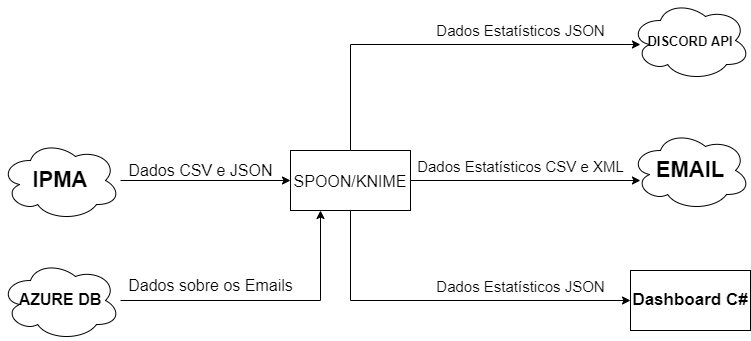
\includegraphics[scale=0.45]{imagens/Scheme.png}
    \caption{Esquema do processo de ETL}
\end{figure}

\vfill
\footnotesize{\textbf{Palavras-chave \\- API} (Application Programming Interface)}
\footnotesize{\textbf{\\- IPMA} (Instituto Português do Mar e da Atmosfera)}